\definecolor{aa}{rgb}{0.00000   0.44700   0.74100}
\definecolor{ab}{rgb}{0.85000   0.32500   0.09800}
\definecolor{ac}{rgb}{1.00000   0.00000   1.00000}
\definecolor{gg}{RGB}{156 156 156}

% GNUPLOT: LaTeX picture with Postscript
\begingroup
  \makeatletter
  \providecommand\color[2][]{%
    \GenericError{(gnuplot) \space\space\space\@spaces}{%
      Package color not loaded in conjunction with
      terminal option `colourtext'%
    }{See the gnuplot documentation for explanation.%
    }{Either use 'blacktext' in gnuplot or load the package
      color.sty in LaTeX.}%
    \renewcommand\color[2][]{}%
  }%
  \providecommand\includegraphics[2][]{%
    \GenericError{(gnuplot) \space\space\space\@spaces}{%
      Package graphicx or graphics not loaded%
    }{See the gnuplot documentation for explanation.%
    }{The gnuplot epslatex terminal needs graphicx.sty or graphics.sty.}%
    \renewcommand\includegraphics[2][]{}%
  }%
  \providecommand\rotatebox[2]{#2}%
  \@ifundefined{ifGPcolor}{%
    \newif\ifGPcolor
    \GPcolorfalse
  }{}%
  \@ifundefined{ifGPblacktext}{%
    \newif\ifGPblacktext
    \GPblacktexttrue
  }{}%
  % define a \g@addto@macro without @ in the name:
  \let\gplgaddtomacro\g@addto@macro
  % define empty templates for all commands taking text:
  \gdef\gplfronttext{}%
  \gdef\gplfronttext{}%
  \makeatother
  \ifGPblacktext
    % no textcolor at all
    \def\colorrgb#1{}%
    \def\colorgray#1{}%
  \else
    % gray or color?
    \ifGPcolor
      \def\colorrgb#1{\color[rgb]{#1}}%
      \def\colorgray#1{\color[gray]{#1}}%
      \expandafter\def\csname LTw\endcsname{\color{white}}%
      \expandafter\def\csname LTb\endcsname{\color{black}}%
      \expandafter\def\csname LTa\endcsname{\color{black}}%
      \expandafter\def\csname LT0\endcsname{\color[rgb]{1,0,0}}%
      \expandafter\def\csname LT1\endcsname{\color[rgb]{0,1,0}}%
      \expandafter\def\csname LT2\endcsname{\color[rgb]{0,0,1}}%
      \expandafter\def\csname LT3\endcsname{\color[rgb]{1,0,1}}%
      \expandafter\def\csname LT4\endcsname{\color[rgb]{0,1,1}}%
      \expandafter\def\csname LT5\endcsname{\color[rgb]{1,1,0}}%
      \expandafter\def\csname LT6\endcsname{\color[rgb]{0,0,0}}%
      \expandafter\def\csname LT7\endcsname{\color[rgb]{1,0.3,0}}%
      \expandafter\def\csname LT8\endcsname{\color[rgb]{0.5,0.5,0.5}}%
    \else
      % gray
      \def\colorrgb#1{\color{black}}%
      \def\colorgray#1{\color[gray]{#1}}%
      \expandafter\def\csname LTw\endcsname{\color{white}}%
      \expandafter\def\csname LTb\endcsname{\color{black}}%
      \expandafter\def\csname LTa\endcsname{\color{black}}%
      \expandafter\def\csname LT0\endcsname{\color{black}}%
      \expandafter\def\csname LT1\endcsname{\color{black}}%
      \expandafter\def\csname LT2\endcsname{\color{black}}%
      \expandafter\def\csname LT3\endcsname{\color{black}}%
      \expandafter\def\csname LT4\endcsname{\color{black}}%
      \expandafter\def\csname LT5\endcsname{\color{black}}%
      \expandafter\def\csname LT6\endcsname{\color{black}}%
      \expandafter\def\csname LT7\endcsname{\color{black}}%
      \expandafter\def\csname LT8\endcsname{\color{black}}%
    \fi
  \fi
    \setlength{\unitlength}{0.0500bp}%
    \ifx\gptboxheight\undefined%
      \newlength{\gptboxheight}%
      \newlength{\gptboxwidth}%
      \newsavebox{\gptboxtext}%
    \fi%
    \setlength{\fboxrule}{0.5pt}%
    \setlength{\fboxsep}{1pt}%
\begin{picture}(8000.00,12000.00)%
    \gplgaddtomacro\gplfronttext{%
      \put(2000,11500){\makebox(0,0){\strut{}{\color{aa}{\rule[0.6mm]{0.5cm}{0.5mm}}} PLICP}}
      \put(4000,11500){\makebox(0,0){\strut{}{\color{ab}{\rule[0.6mm]{0.5cm}{0.5mm}}} NDT}}
      \put(6000,11500){\makebox(0,0){\strut{}{\color{ac}{\rule[0.6mm]{0.5cm}{0.5mm}}} \texttt{fsm}}}
    }%
    \gplgaddtomacro\gplfronttext{%
      \colorrgb{0.15,0.15,0.15}%
      \put(79,10799){\makebox(0,0)[r]{\strut{}$21.0$}}%
      \colorrgb{0.15,0.15,0.15}%
      \put(79,9908){\makebox(0,0)[r]{\strut{}$19.0$}}%
      \colorrgb{0.15,0.15,0.15}%
      \put(79,9017){\makebox(0,0)[r]{\strut{}$17.0$}}%
      \colorrgb{0.15,0.15,0.15}%
      \put(79,8126){\makebox(0,0)[r]{\strut{}$15.0$}}%
      \colorrgb{0.15,0.15,0.15}%
      \put(657,11019){\makebox(0,0){\strut{}$12.0$}}%
      \colorrgb{0.15,0.15,0.15}%
      \put(2439,11019){\makebox(0,0){\strut{}$16.0$}}%
      \colorrgb{0.15,0.15,0.15}%
      \put(4222,11019){\makebox(0,0){\strut{}$20.0$}}%
      \colorrgb{0.15,0.15,0.15}%
      \put(6004,11019){\makebox(0,0){\strut{}$24.0$}}%
      \colorrgb{0.15,0.15,0.15}%
      \put(7787,11019){\makebox(0,0){\strut{}$28.0$}}%

      \put(6004,8126){\makebox(0,0)     {\color{gg}{\strut{}$\bigotimes_0$}}}      % (x_24, y_15)
      \put(4222,9462.5){\makebox(0,0)   {\color{gg}{\strut{}$\bigotimes_1$}}}      % (x_20, y_18)
      \put(5558.5,10353.5){\makebox(0,0){\color{gg}{\strut{}$\bigotimes_2$}}}      % (x_23, y_20)
      \put(6895.5,9562.5){\makebox(0,0) {\color{gg}{\strut{}$\bigotimes_3$}}}      % (x_26, y_18)
      \put(4667.5,8571.5){\makebox(0,0) {\color{gg}{\strut{}$\bigotimes_4$}}}      % (x_21, y_16)
      \put(1431,8571.5){\makebox(0,0)   {\color{gg}{\strut{}$\bigotimes_5$}}}      % (x_13, y_16)
    }%
    \gplgaddtomacro\gplfronttext{%
    }%
    \gplgaddtomacro\gplfronttext{%
      \colorrgb{0.15,0.15,0.15}%
      \put(79,7559){\makebox(0,0)[r]{\strut{}$21.0$}}%
      \colorrgb{0.15,0.15,0.15}%
      \put(79,6668){\makebox(0,0)[r]{\strut{}$19.0$}}%
      \colorrgb{0.15,0.15,0.15}%
      \put(79,5777){\makebox(0,0)[r]{\strut{}$17.0$}}%
      \colorrgb{0.15,0.15,0.15}%
      \put(79,4886){\makebox(0,0)[r]{\strut{}$15.0$}}%
      \colorrgb{0.15,0.15,0.15}%
      \put(657,4220){\makebox(0,0){\strut{}}}%
      \colorrgb{0.15,0.15,0.15}%
      \put(2439,4220){\makebox(0,0){\strut{}}}%
      \colorrgb{0.15,0.15,0.15}%
      \put(4222,4220){\makebox(0,0){\strut{}}}%
      \colorrgb{0.15,0.15,0.15}%
      \put(6004,4220){\makebox(0,0){\strut{}}}%
      \colorrgb{0.15,0.15,0.15}%
      \put(7787,4220){\makebox(0,0){\strut{}}}%

      \put(6004,4886){\makebox(0,0)    {\color{gg}{\strut{}$\bigotimes_0$}}}      % (x_24, y_15)
      \put(4222,6222.5){\makebox(0,0)  {\color{gg}{\strut{}$\bigotimes_1$}}}      % (x_20, y_18)
      \put(5558.5,7113.5){\makebox(0,0){\color{gg}{\strut{}$\bigotimes_2$}}}      % (x_23, y_20)
      \put(6895.5,6322.5){\makebox(0,0){\color{gg}{\strut{}$\bigotimes_3$}}}      % (x_26, y_18)
      \put(4667.5,5331.5){\makebox(0,0){\color{gg}{\strut{}$\bigotimes_4$}}}      % (x_21, y_16)
      \put(1431,5331.5){\makebox(0,0)  {\color{gg}{\strut{}$\bigotimes_5$}}}      % (x_13, y_16)
    }%
    \gplgaddtomacro\gplfronttext{%
    }%
    \gplgaddtomacro\gplfronttext{%
      \colorrgb{0.15,0.15,0.15}%
      \put(79,4319){\makebox(0,0)[r]{\strut{}$21.0$}}%
      \colorrgb{0.15,0.15,0.15}%
      \put(79,3428){\makebox(0,0)[r]{\strut{}$19.0$}}%
      \colorrgb{0.15,0.15,0.15}%
      \put(79,2537){\makebox(0,0)[r]{\strut{}$17.0$}}%
      \colorrgb{0.15,0.15,0.15}%
      \put(79,1646){\makebox(0,0)[r]{\strut{}$15.0$}}%
      \colorrgb{0.15,0.15,0.15}%
      \put(657,980){\makebox(0,0){\strut{}$12.0$}}%
      \colorrgb{0.15,0.15,0.15}%
      \put(2439,980){\makebox(0,0){\strut{}$16.0$}}%
      \colorrgb{0.15,0.15,0.15}%
      \put(4222,980){\makebox(0,0){\strut{}$20.0$}}%
      \colorrgb{0.15,0.15,0.15}%
      \put(6004,980){\makebox(0,0){\strut{}$24.0$}}%
      \colorrgb{0.15,0.15,0.15}%
      \put(7787,980){\makebox(0,0){\strut{}$28.0$}}%

      \put(6004,1646){\makebox(0,0)    {\color{gg}{\strut{}$\bigotimes_0$}}}      % (x_24, y_15)
      \put(4222,2932.5){\makebox(0,0)  {\color{gg}{\strut{}$\bigotimes_1$}}}      % (x_20, y_18)
      \put(5558.5,3873.5){\makebox(0,0){\color{gg}{\strut{}$\bigotimes_2$}}}      % (x_23, y_20)
      \put(6895.5,3032.5){\makebox(0,0){\color{gg}{\strut{}$\bigotimes_3$}}}      % (x_26, y_18)
      \put(4667.5,2091.5){\makebox(0,0){\color{gg}{\strut{}$\bigotimes_4$}}}      % (x_21, y_16)
      \put(1431,2091.5){\makebox(0,0)  {\color{gg}{\strut{}$\bigotimes_5$}}}      % (x_13, y_16)
    }%
    \put(0,0){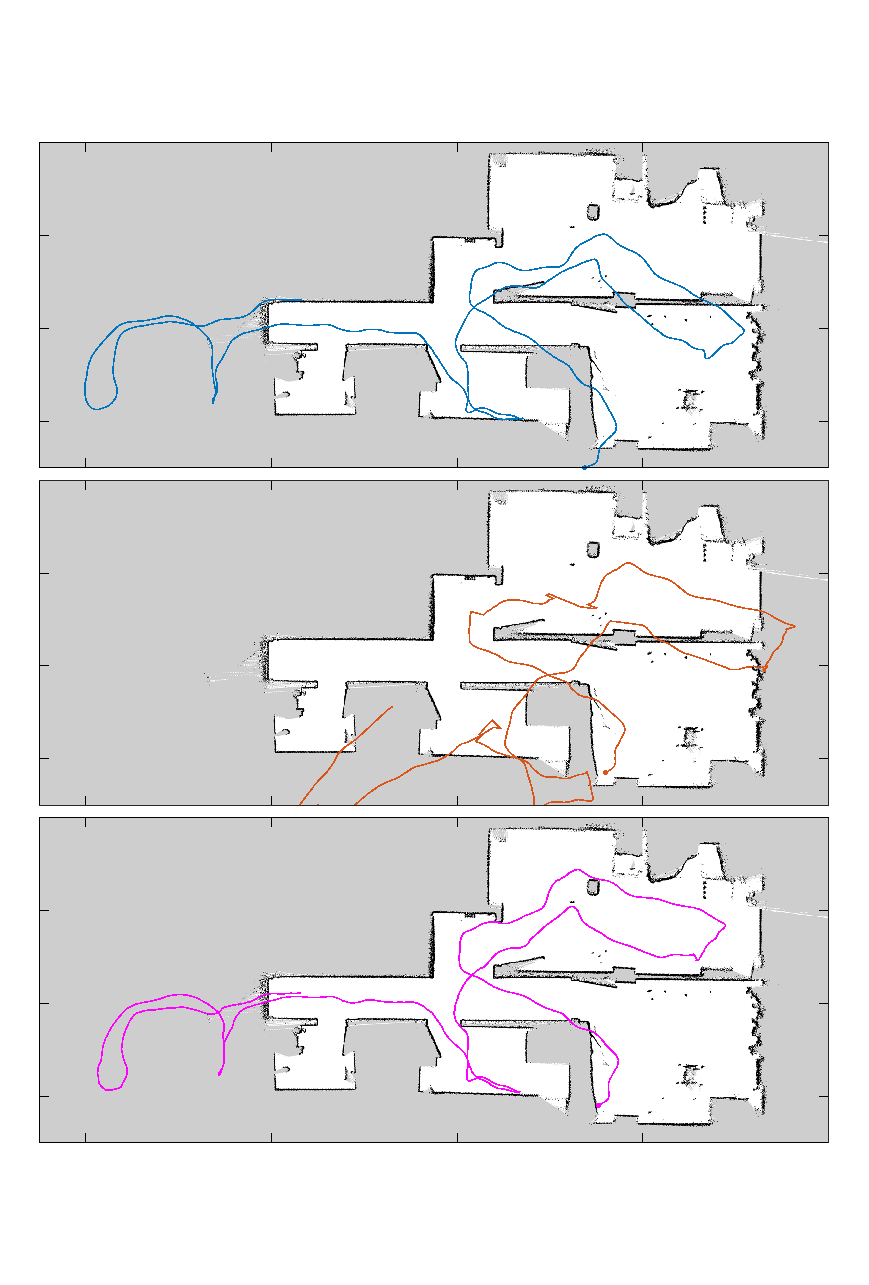
\includegraphics{./figures/parts/02/chapters/05/sections/04/odom_test}}%
    \gplfronttext
  \end{picture}%
\endgroup
